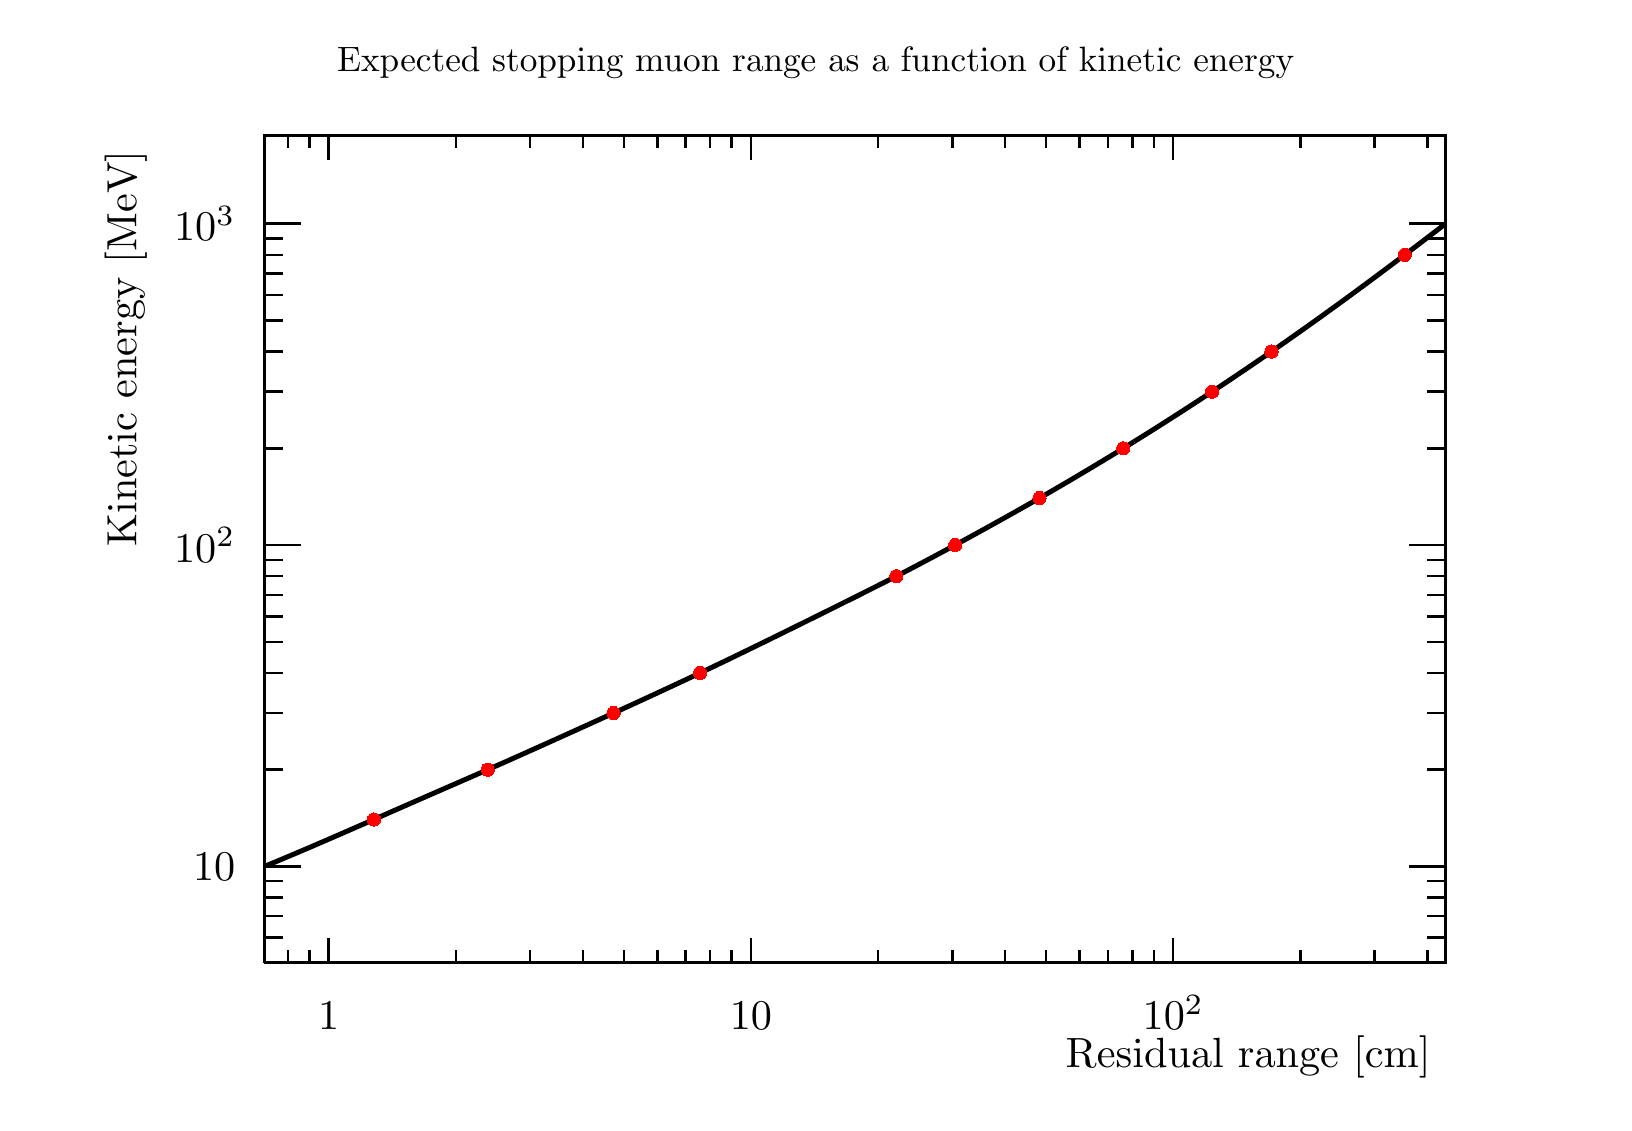
\begin{tikzpicture}
\pgfdeclareplotmark{cross} {
\pgfpathmoveto{\pgfpoint{-0.3\pgfplotmarksize}{\pgfplotmarksize}}
\pgfpathlineto{\pgfpoint{+0.3\pgfplotmarksize}{\pgfplotmarksize}}
\pgfpathlineto{\pgfpoint{+0.3\pgfplotmarksize}{0.3\pgfplotmarksize}}
\pgfpathlineto{\pgfpoint{+1\pgfplotmarksize}{0.3\pgfplotmarksize}}
\pgfpathlineto{\pgfpoint{+1\pgfplotmarksize}{-0.3\pgfplotmarksize}}
\pgfpathlineto{\pgfpoint{+0.3\pgfplotmarksize}{-0.3\pgfplotmarksize}}
\pgfpathlineto{\pgfpoint{+0.3\pgfplotmarksize}{-1.\pgfplotmarksize}}
\pgfpathlineto{\pgfpoint{-0.3\pgfplotmarksize}{-1.\pgfplotmarksize}}
\pgfpathlineto{\pgfpoint{-0.3\pgfplotmarksize}{-0.3\pgfplotmarksize}}
\pgfpathlineto{\pgfpoint{-1.\pgfplotmarksize}{-0.3\pgfplotmarksize}}
\pgfpathlineto{\pgfpoint{-1.\pgfplotmarksize}{0.3\pgfplotmarksize}}
\pgfpathlineto{\pgfpoint{-0.3\pgfplotmarksize}{0.3\pgfplotmarksize}}
\pgfpathclose
\pgfusepathqstroke
}
\pgfdeclareplotmark{cross*} {
\pgfpathmoveto{\pgfpoint{-0.3\pgfplotmarksize}{\pgfplotmarksize}}
\pgfpathlineto{\pgfpoint{+0.3\pgfplotmarksize}{\pgfplotmarksize}}
\pgfpathlineto{\pgfpoint{+0.3\pgfplotmarksize}{0.3\pgfplotmarksize}}
\pgfpathlineto{\pgfpoint{+1\pgfplotmarksize}{0.3\pgfplotmarksize}}
\pgfpathlineto{\pgfpoint{+1\pgfplotmarksize}{-0.3\pgfplotmarksize}}
\pgfpathlineto{\pgfpoint{+0.3\pgfplotmarksize}{-0.3\pgfplotmarksize}}
\pgfpathlineto{\pgfpoint{+0.3\pgfplotmarksize}{-1.\pgfplotmarksize}}
\pgfpathlineto{\pgfpoint{-0.3\pgfplotmarksize}{-1.\pgfplotmarksize}}
\pgfpathlineto{\pgfpoint{-0.3\pgfplotmarksize}{-0.3\pgfplotmarksize}}
\pgfpathlineto{\pgfpoint{-1.\pgfplotmarksize}{-0.3\pgfplotmarksize}}
\pgfpathlineto{\pgfpoint{-1.\pgfplotmarksize}{0.3\pgfplotmarksize}}
\pgfpathlineto{\pgfpoint{-0.3\pgfplotmarksize}{0.3\pgfplotmarksize}}
\pgfpathclose
\pgfusepathqfillstroke
}
\pgfdeclareplotmark{newstar} {
\pgfpathmoveto{\pgfqpoint{0pt}{\pgfplotmarksize}}
\pgfpathlineto{\pgfqpointpolar{44}{0.5\pgfplotmarksize}}
\pgfpathlineto{\pgfqpointpolar{18}{\pgfplotmarksize}}
\pgfpathlineto{\pgfqpointpolar{-20}{0.5\pgfplotmarksize}}
\pgfpathlineto{\pgfqpointpolar{-54}{\pgfplotmarksize}}
\pgfpathlineto{\pgfqpointpolar{-90}{0.5\pgfplotmarksize}}
\pgfpathlineto{\pgfqpointpolar{234}{\pgfplotmarksize}}
\pgfpathlineto{\pgfqpointpolar{198}{0.5\pgfplotmarksize}}
\pgfpathlineto{\pgfqpointpolar{162}{\pgfplotmarksize}}
\pgfpathlineto{\pgfqpointpolar{134}{0.5\pgfplotmarksize}}
\pgfpathclose
\pgfusepathqstroke
}
\pgfdeclareplotmark{newstar*} {
\pgfpathmoveto{\pgfqpoint{0pt}{\pgfplotmarksize}}
\pgfpathlineto{\pgfqpointpolar{44}{0.5\pgfplotmarksize}}
\pgfpathlineto{\pgfqpointpolar{18}{\pgfplotmarksize}}
\pgfpathlineto{\pgfqpointpolar{-20}{0.5\pgfplotmarksize}}
\pgfpathlineto{\pgfqpointpolar{-54}{\pgfplotmarksize}}
\pgfpathlineto{\pgfqpointpolar{-90}{0.5\pgfplotmarksize}}
\pgfpathlineto{\pgfqpointpolar{234}{\pgfplotmarksize}}
\pgfpathlineto{\pgfqpointpolar{198}{0.5\pgfplotmarksize}}
\pgfpathlineto{\pgfqpointpolar{162}{\pgfplotmarksize}}
\pgfpathlineto{\pgfqpointpolar{134}{0.5\pgfplotmarksize}}
\pgfpathclose
\pgfusepathqfillstroke
}
\definecolor{c}{rgb}{1,1,1};
\draw [color=c, fill=c] (0,0) rectangle (20,13.639);
\draw [color=c, fill=c] (3,1.77307) rectangle (18,12.2751);
\definecolor{c}{rgb}{0,0,0};
\draw [c,line width=0.9] (3,1.77307) -- (3,12.2751) -- (18,12.2751) -- (18,1.77307) -- (3,1.77307);
\definecolor{c}{rgb}{1,1,1};
\draw [color=c, fill=c] (0,0) rectangle (20,13.639);
\draw [color=c, fill=c] (3,1.77307) rectangle (18,12.2751);
\definecolor{c}{rgb}{0,0,0};
\draw [c,line width=0.9] (3,1.77307) -- (3,12.2751) -- (18,12.2751) -- (18,1.77307) -- (3,1.77307);
\draw [c,line width=1.8] (3.01883,3.00168) -- (3.05633,3.01716) -- (3.09383,3.03268) -- (3.13133,3.04826) -- (3.16883,3.06388) -- (3.20633,3.07955) -- (3.24383,3.09526) -- (3.28133,3.11102) -- (3.31883,3.12682) -- (3.35633,3.14266) --
 (3.39383,3.15854) -- (3.43133,3.17446) -- (3.46883,3.19042) -- (3.50633,3.20641) -- (3.54383,3.22244) -- (3.58133,3.2385) -- (3.61883,3.25459) -- (3.65633,3.27071) -- (3.69383,3.28686) -- (3.73133,3.30304) -- (3.76883,3.31925) -- (3.80633,3.33548)
 -- (3.84383,3.35173) -- (3.88133,3.36801) -- (3.91883,3.38431) -- (3.95633,3.40063) -- (3.99383,3.41696) -- (4.03133,3.43332) -- (4.06883,3.44968) -- (4.10633,3.46607) -- (4.14383,3.48246) -- (4.18133,3.49887) -- (4.21883,3.51529) --
 (4.25633,3.53172) -- (4.29383,3.54816) -- (4.33133,3.5646) -- (4.36883,3.58105) -- (4.40633,3.59751) -- (4.44383,3.61397) -- (4.48133,3.63043) -- (4.51883,3.64689) -- (4.55633,3.66335) -- (4.59383,3.67982) -- (4.63133,3.69628) -- (4.66883,3.71274)
 -- (4.70633,3.72919) -- (4.74383,3.74565) -- (4.78133,3.7621) -- (4.81883,3.77854) -- (4.85633,3.79498);
\draw [c,line width=1.8] (4.85633,3.79498) -- (4.89383,3.81141) -- (4.93133,3.82784) -- (4.96883,3.84426) -- (5.00633,3.86067) -- (5.04383,3.87707) -- (5.08133,3.89347) -- (5.11883,3.90986) -- (5.15633,3.92625) -- (5.19383,3.94262) -- (5.23133,3.959)
 -- (5.26883,3.97536) -- (5.30633,3.99172) -- (5.34383,4.00808) -- (5.38133,4.02444) -- (5.41883,4.04079) -- (5.45633,4.05714) -- (5.49383,4.0735) -- (5.53133,4.08985) -- (5.56883,4.10621) -- (5.60633,4.12258) -- (5.64383,4.13896) --
 (5.68133,4.15535) -- (5.71883,4.17176) -- (5.75633,4.18818) -- (5.79383,4.20463) -- (5.83133,4.2211) -- (5.86883,4.2376) -- (5.90633,4.25413) -- (5.94383,4.27069) -- (5.98133,4.28727) -- (6.01883,4.30388) -- (6.05633,4.32052) -- (6.09383,4.33717) --
 (6.13133,4.35385) -- (6.16883,4.37055) -- (6.20633,4.38728) -- (6.24383,4.40402) -- (6.28133,4.42077) -- (6.31883,4.43755) -- (6.35633,4.45434) -- (6.39383,4.47115) -- (6.43133,4.48797) -- (6.46883,4.50481) -- (6.50633,4.52165) -- (6.54383,4.53851)
 -- (6.58133,4.55538) -- (6.61883,4.57227) -- (6.65633,4.58916) -- (6.69383,4.60606);
\draw [c,line width=1.8] (6.69383,4.60606) -- (6.73133,4.62297) -- (6.76883,4.63989) -- (6.80633,4.65682) -- (6.84383,4.67375) -- (6.88133,4.6907) -- (6.91883,4.70765) -- (6.95633,4.72461) -- (6.99383,4.74157) -- (7.03133,4.75855) --
 (7.06883,4.77553) -- (7.10633,4.79252) -- (7.14383,4.80952) -- (7.18133,4.82653) -- (7.21883,4.84356) -- (7.25633,4.86059) -- (7.29383,4.87764) -- (7.33133,4.89469) -- (7.36883,4.91177) -- (7.40633,4.92886) -- (7.44383,4.94597) -- (7.48133,4.9631)
 -- (7.51883,4.98025) -- (7.55633,4.99741) -- (7.59383,5.0146) -- (7.63133,5.0318) -- (7.66883,5.04902) -- (7.70633,5.06626) -- (7.74383,5.08351) -- (7.78133,5.10078) -- (7.81883,5.11806) -- (7.85633,5.13537) -- (7.89383,5.15268) -- (7.93133,5.17002)
 -- (7.96883,5.18737) -- (8.00633,5.20474) -- (8.04383,5.22213) -- (8.08133,5.23954) -- (8.11883,5.25696) -- (8.15633,5.27441) -- (8.19383,5.29188) -- (8.23133,5.30936) -- (8.26883,5.32688) -- (8.30633,5.34442) -- (8.34383,5.36198) --
 (8.38133,5.37957) -- (8.41883,5.3972) -- (8.45633,5.41485) -- (8.49383,5.43254) -- (8.53133,5.45027);
\draw [c,line width=1.8] (8.53133,5.45027) -- (8.56883,5.46804) -- (8.60633,5.48585) -- (8.64383,5.50369) -- (8.68133,5.52157) -- (8.71883,5.53949) -- (8.75633,5.55744) -- (8.79383,5.57543) -- (8.83133,5.59345) -- (8.86883,5.6115) --
 (8.90633,5.62958) -- (8.94383,5.64769) -- (8.98133,5.66582) -- (9.01883,5.68399) -- (9.05633,5.70218) -- (9.09383,5.72039) -- (9.13133,5.73863) -- (9.16883,5.75689) -- (9.20633,5.77517) -- (9.24383,5.79348) -- (9.28133,5.8118) -- (9.31883,5.83014)
 -- (9.35633,5.8485) -- (9.39383,5.86688) -- (9.43133,5.88527) -- (9.46883,5.90368) -- (9.50633,5.9221) -- (9.54383,5.94054) -- (9.58133,5.95899) -- (9.61883,5.97745) -- (9.65633,5.99593) -- (9.69383,6.01441) -- (9.73133,6.03291) -- (9.76883,6.05142)
 -- (9.80633,6.06994) -- (9.84383,6.08846) -- (9.88133,6.107) -- (9.91883,6.12555) -- (9.95633,6.1441) -- (9.99383,6.16267) -- (10.0313,6.18124) -- (10.0688,6.19983) -- (10.1063,6.21842) -- (10.1438,6.23702) -- (10.1813,6.25564) -- (10.2188,6.27426)
 -- (10.2563,6.2929) -- (10.2938,6.31154) -- (10.3313,6.3302) -- (10.3688,6.34888);
\draw [c,line width=1.8] (10.3688,6.34888) -- (10.4063,6.36757) -- (10.4438,6.38628) -- (10.4813,6.405) -- (10.5188,6.42374) -- (10.5563,6.44251) -- (10.5938,6.4613) -- (10.6313,6.48011) -- (10.6688,6.49895) -- (10.7063,6.51782) -- (10.7438,6.53673)
 -- (10.7813,6.55567) -- (10.8188,6.57464) -- (10.8563,6.59366) -- (10.8938,6.61273) -- (10.9313,6.63185) -- (10.9688,6.65102) -- (11.0063,6.67025) -- (11.0438,6.68954) -- (11.0813,6.7089) -- (11.1188,6.72832) -- (11.1563,6.7478) -- (11.1938,6.76735)
 -- (11.2313,6.78695) -- (11.2688,6.80662) -- (11.3063,6.82634) -- (11.3438,6.84611) -- (11.3813,6.86594) -- (11.4188,6.88583) -- (11.4563,6.90577) -- (11.4938,6.92575) -- (11.5313,6.94579) -- (11.5688,6.96587) -- (11.6063,6.986) -- (11.6438,7.00617)
 -- (11.6813,7.02639) -- (11.7188,7.04665) -- (11.7563,7.06694) -- (11.7938,7.08728) -- (11.8313,7.10765) -- (11.8688,7.12806) -- (11.9063,7.14851) -- (11.9438,7.16899) -- (11.9813,7.18951) -- (12.0188,7.21006) -- (12.0563,7.23065) --
 (12.0938,7.25128) -- (12.1313,7.27194) -- (12.1688,7.29264) -- (12.2063,7.31338);
\draw [c,line width=1.8] (12.2063,7.31338) -- (12.2438,7.33416) -- (12.2813,7.35497) -- (12.3188,7.37582) -- (12.3563,7.39671) -- (12.3938,7.41764) -- (12.4313,7.4386) -- (12.4688,7.45961) -- (12.5063,7.48066) -- (12.5438,7.50176) --
 (12.5813,7.52289) -- (12.6188,7.54408) -- (12.6563,7.5653) -- (12.6938,7.58658) -- (12.7313,7.60791) -- (12.7688,7.62928) -- (12.8063,7.65071) -- (12.8438,7.67219) -- (12.8813,7.69374) -- (12.9188,7.71533) -- (12.9563,7.73698) -- (12.9938,7.75869)
 -- (13.0313,7.78046) -- (13.0688,7.80227) -- (13.1063,7.82415) -- (13.1438,7.84607) -- (13.1813,7.86806) -- (13.2188,7.89009) -- (13.2563,7.91218) -- (13.2938,7.93432) -- (13.3313,7.95652) -- (13.3688,7.97877) -- (13.4063,8.00107) --
 (13.4438,8.02342) -- (13.4813,8.04583) -- (13.5188,8.06829) -- (13.5563,8.09081) -- (13.5938,8.11338) -- (13.6313,8.136) -- (13.6688,8.15868) -- (13.7063,8.18141) -- (13.7438,8.20419) -- (13.7813,8.22704) -- (13.8188,8.24993) -- (13.8563,8.27289) --
 (13.8938,8.2959) -- (13.9313,8.31897) -- (13.9688,8.3421) -- (14.0063,8.36528) -- (14.0438,8.38852);
\draw [c,line width=1.8] (14.0438,8.38852) -- (14.0813,8.41182) -- (14.1188,8.43518) -- (14.1563,8.45859) -- (14.1938,8.48206) -- (14.2313,8.50558) -- (14.2688,8.52916) -- (14.3063,8.55279) -- (14.3438,8.57648) -- (14.3813,8.60023) --
 (14.4188,8.62403) -- (14.4563,8.64788) -- (14.4938,8.67179) -- (14.5313,8.69575) -- (14.5688,8.71977) -- (14.6063,8.74385) -- (14.6438,8.76797) -- (14.6813,8.79216) -- (14.7188,8.8164) -- (14.7563,8.84069) -- (14.7938,8.86504) -- (14.8313,8.88945)
 -- (14.8688,8.91391) -- (14.9063,8.93843) -- (14.9438,8.96301) -- (14.9813,8.98765) -- (15.0188,9.01234) -- (15.0563,9.03709) -- (15.0938,9.0619) -- (15.1313,9.08677) -- (15.1688,9.1117) -- (15.2063,9.13669) -- (15.2438,9.16174) -- (15.2813,9.18684)
 -- (15.3188,9.21201) -- (15.3563,9.23723) -- (15.3938,9.26252) -- (15.4313,9.28786) -- (15.4688,9.31326) -- (15.5063,9.33872) -- (15.5438,9.36424) -- (15.5813,9.38982) -- (15.6188,9.41546) -- (15.6563,9.44116) -- (15.6938,9.46692) --
 (15.7313,9.49275) -- (15.7688,9.51863) -- (15.8063,9.54458) -- (15.8438,9.57059) -- (15.8813,9.59666);
\draw [c,line width=1.8] (15.8813,9.59666) -- (15.9188,9.62279) -- (15.9563,9.64898) -- (15.9938,9.67524) -- (16.0313,9.70155) -- (16.0688,9.72792) -- (16.1063,9.75436) -- (16.1438,9.78085) -- (16.1813,9.8074) -- (16.2188,9.834) -- (16.2563,9.86067)
 -- (16.2938,9.88739) -- (16.3313,9.91416) -- (16.3688,9.941) -- (16.4063,9.96789) -- (16.4438,9.99483) -- (16.4813,10.0218) -- (16.5188,10.0489) -- (16.5563,10.076) -- (16.5938,10.1031) -- (16.6313,10.1304) -- (16.6688,10.1576) -- (16.7063,10.1849)
 -- (16.7438,10.2123) -- (16.7813,10.2397) -- (16.8188,10.2672) -- (16.8563,10.2947) -- (16.8938,10.3223) -- (16.9313,10.3499) -- (16.9688,10.3776) -- (17.0063,10.4053) -- (17.0438,10.4331) -- (17.0813,10.4609) -- (17.1188,10.4888) --
 (17.1563,10.5167) -- (17.1938,10.5447) -- (17.2313,10.5727) -- (17.2688,10.6008) -- (17.3063,10.6289) -- (17.3438,10.657) -- (17.3813,10.6852) -- (17.4188,10.7135) -- (17.4563,10.7418) -- (17.4938,10.7701) -- (17.5313,10.7985) -- (17.5688,10.8269)
 -- (17.6063,10.8554) -- (17.6438,10.8839) -- (17.6813,10.9124) -- (17.7188,10.941);
\draw [c,line width=1.8] (17.7188,10.941) -- (17.7563,10.9696) -- (17.7938,10.9983) -- (17.8313,11.027) -- (17.8688,11.0558) -- (17.9063,11.0846) -- (17.9438,11.1134) -- (17.9813,11.1423);
\draw [c,line width=0.9] (3,1.77307) -- (18,1.77307);
\draw [c,line width=0.9] (3.2965,1.9265) -- (3.2965,1.77307);
\draw [c,line width=0.9] (3.57082,1.9265) -- (3.57082,1.77307);
\draw [c,line width=0.9] (3.8162,2.07994) -- (3.8162,1.77307);
\draw [anchor=base] (3.8162,0.92063) node[scale=1.52731, color=c, rotate=0]{1};
\draw [c,line width=0.9] (5.43053,1.9265) -- (5.43053,1.77307);
\draw [c,line width=0.9] (6.37485,1.9265) -- (6.37485,1.77307);
\draw [c,line width=0.9] (7.04486,1.9265) -- (7.04486,1.77307);
\draw [c,line width=0.9] (7.56456,1.9265) -- (7.56456,1.77307);
\draw [c,line width=0.9] (7.98918,1.9265) -- (7.98918,1.77307);
\draw [c,line width=0.9] (8.34819,1.9265) -- (8.34819,1.77307);
\draw [c,line width=0.9] (8.65919,1.9265) -- (8.65919,1.77307);
\draw [c,line width=0.9] (8.9335,1.9265) -- (8.9335,1.77307);
\draw [c,line width=0.9] (9.17888,2.07994) -- (9.17888,1.77307);
\draw [anchor=base] (9.17888,0.92063) node[scale=1.52731, color=c, rotate=0]{10};
\draw [c,line width=0.9] (10.7932,1.9265) -- (10.7932,1.77307);
\draw [c,line width=0.9] (11.7375,1.9265) -- (11.7375,1.77307);
\draw [c,line width=0.9] (12.4075,1.9265) -- (12.4075,1.77307);
\draw [c,line width=0.9] (12.9272,1.9265) -- (12.9272,1.77307);
\draw [c,line width=0.9] (13.3519,1.9265) -- (13.3519,1.77307);
\draw [c,line width=0.9] (13.7109,1.9265) -- (13.7109,1.77307);
\draw [c,line width=0.9] (14.0219,1.9265) -- (14.0219,1.77307);
\draw [c,line width=0.9] (14.2962,1.9265) -- (14.2962,1.77307);
\draw [c,line width=0.9] (14.5416,2.07994) -- (14.5416,1.77307);
\draw [anchor=base] (14.5416,0.92063) node[scale=1.52731, color=c, rotate=0]{$10^{2}$};
\draw [c,line width=0.9] (16.1559,1.9265) -- (16.1559,1.77307);
\draw [c,line width=0.9] (17.1002,1.9265) -- (17.1002,1.77307);
\draw [c,line width=0.9] (17.7702,1.9265) -- (17.7702,1.77307);
\draw [anchor= east] (18,0.572837) node[scale=1.52731, color=c, rotate=0]{ Residual range [cm]};
\draw [c,line width=0.9] (3,12.2751) -- (18,12.2751);
\draw [c,line width=0.9] (3.2965,12.1216) -- (3.2965,12.2751);
\draw [c,line width=0.9] (3.57082,12.1216) -- (3.57082,12.2751);
\draw [c,line width=0.9] (3.8162,11.9682) -- (3.8162,12.2751);
\draw [c,line width=0.9] (5.43053,12.1216) -- (5.43053,12.2751);
\draw [c,line width=0.9] (6.37485,12.1216) -- (6.37485,12.2751);
\draw [c,line width=0.9] (7.04486,12.1216) -- (7.04486,12.2751);
\draw [c,line width=0.9] (7.56456,12.1216) -- (7.56456,12.2751);
\draw [c,line width=0.9] (7.98918,12.1216) -- (7.98918,12.2751);
\draw [c,line width=0.9] (8.34819,12.1216) -- (8.34819,12.2751);
\draw [c,line width=0.9] (8.65919,12.1216) -- (8.65919,12.2751);
\draw [c,line width=0.9] (8.9335,12.1216) -- (8.9335,12.2751);
\draw [c,line width=0.9] (9.17888,11.9682) -- (9.17888,12.2751);
\draw [c,line width=0.9] (10.7932,12.1216) -- (10.7932,12.2751);
\draw [c,line width=0.9] (11.7375,12.1216) -- (11.7375,12.2751);
\draw [c,line width=0.9] (12.4075,12.1216) -- (12.4075,12.2751);
\draw [c,line width=0.9] (12.9272,12.1216) -- (12.9272,12.2751);
\draw [c,line width=0.9] (13.3519,12.1216) -- (13.3519,12.2751);
\draw [c,line width=0.9] (13.7109,12.1216) -- (13.7109,12.2751);
\draw [c,line width=0.9] (14.0219,12.1216) -- (14.0219,12.2751);
\draw [c,line width=0.9] (14.2962,12.1216) -- (14.2962,12.2751);
\draw [c,line width=0.9] (14.5416,11.9682) -- (14.5416,12.2751);
\draw [c,line width=0.9] (16.1559,12.1216) -- (16.1559,12.2751);
\draw [c,line width=0.9] (17.1002,12.1216) -- (17.1002,12.2751);
\draw [c,line width=0.9] (17.7702,12.1216) -- (17.7702,12.2751);
\draw [c,line width=0.9] (3,1.77307) -- (3,12.2751);
\draw [c,line width=0.9] (3.231,2.08848) -- (3,2.08848);
\draw [c,line width=0.9] (3.231,2.36172) -- (3,2.36172);
\draw [c,line width=0.9] (3.231,2.5984) -- (3,2.5984);
\draw [c,line width=0.9] (3.231,2.80718) -- (3,2.80718);
\draw [c,line width=0.9] (3.462,2.99393) -- (3,2.99393);
\draw [anchor= east] (2.82,2.99393) node[scale=1.52731, color=c, rotate=0]{10};
\draw [c,line width=0.9] (3.231,4.22255) -- (3,4.22255);
\draw [c,line width=0.9] (3.231,4.94124) -- (3,4.94124);
\draw [c,line width=0.9] (3.231,5.45116) -- (3,5.45116);
\draw [c,line width=0.9] (3.231,5.84669) -- (3,5.84669);
\draw [c,line width=0.9] (3.231,6.16986) -- (3,6.16986);
\draw [c,line width=0.9] (3.231,6.44309) -- (3,6.44309);
\draw [c,line width=0.9] (3.231,6.67978) -- (3,6.67978);
\draw [c,line width=0.9] (3.231,6.88855) -- (3,6.88855);
\draw [c,line width=0.9] (3.462,7.07531) -- (3,7.07531);
\draw [anchor= east] (2.82,7.07531) node[scale=1.52731, color=c, rotate=0]{$10^{2}$};
\draw [c,line width=0.9] (3.231,8.30392) -- (3,8.30392);
\draw [c,line width=0.9] (3.231,9.02262) -- (3,9.02262);
\draw [c,line width=0.9] (3.231,9.53254) -- (3,9.53254);
\draw [c,line width=0.9] (3.231,9.92807) -- (3,9.92807);
\draw [c,line width=0.9] (3.231,10.2512) -- (3,10.2512);
\draw [c,line width=0.9] (3.231,10.5245) -- (3,10.5245);
\draw [c,line width=0.9] (3.231,10.7612) -- (3,10.7612);
\draw [c,line width=0.9] (3.231,10.9699) -- (3,10.9699);
\draw [c,line width=0.9] (3.462,11.1567) -- (3,11.1567);
\draw [anchor= east] (2.82,11.1567) node[scale=1.52731, color=c, rotate=0]{$10^{3}$};
\draw [anchor= east] (1.24,12.2751) node[scale=1.52731, color=c, rotate=90]{ Kinetic energy [MeV]};
\draw [c,line width=0.9] (18,1.77307) -- (18,12.2751);
\draw [c,line width=0.9] (17.769,2.08848) -- (18,2.08848);
\draw [c,line width=0.9] (17.769,2.36172) -- (18,2.36172);
\draw [c,line width=0.9] (17.769,2.5984) -- (18,2.5984);
\draw [c,line width=0.9] (17.769,2.80718) -- (18,2.80718);
\draw [c,line width=0.9] (17.538,2.99393) -- (18,2.99393);
\draw [c,line width=0.9] (17.769,4.22255) -- (18,4.22255);
\draw [c,line width=0.9] (17.769,4.94124) -- (18,4.94124);
\draw [c,line width=0.9] (17.769,5.45116) -- (18,5.45116);
\draw [c,line width=0.9] (17.769,5.84669) -- (18,5.84669);
\draw [c,line width=0.9] (17.769,6.16986) -- (18,6.16986);
\draw [c,line width=0.9] (17.769,6.44309) -- (18,6.44309);
\draw [c,line width=0.9] (17.769,6.67978) -- (18,6.67978);
\draw [c,line width=0.9] (17.769,6.88855) -- (18,6.88855);
\draw [c,line width=0.9] (17.538,7.07531) -- (18,7.07531);
\draw [c,line width=0.9] (17.769,8.30392) -- (18,8.30392);
\draw [c,line width=0.9] (17.769,9.02262) -- (18,9.02262);
\draw [c,line width=0.9] (17.769,9.53254) -- (18,9.53254);
\draw [c,line width=0.9] (17.769,9.92807) -- (18,9.92807);
\draw [c,line width=0.9] (17.769,10.2512) -- (18,10.2512);
\draw [c,line width=0.9] (17.769,10.5245) -- (18,10.5245);
\draw [c,line width=0.9] (17.769,10.7612) -- (18,10.7612);
\draw [c,line width=0.9] (17.769,10.9699) -- (18,10.9699);
\draw [c,line width=0.9] (17.538,11.1567) -- (18,11.1567);
\definecolor{c}{rgb}{1,0,0};
\foreach \P in {(4.38998,3.59034), (5.83462,4.22255), (7.43347,4.94124), (8.53322,5.45117), (11.0249,6.67978), (11.7718,7.07531), (12.843,7.67171), (13.9069,8.30392), (15.0344,9.02262), (15.7889,9.53254), (17.482,10.7612)}{\draw[mark
 options={color=c,fill=c},mark size=2.402402pt, line width=0.000000pt, mark=*] plot coordinates {\P};}
\definecolor{c}{rgb}{1,1,1};
\draw [color=c, fill=c] (2,12.8206) rectangle (18,13.5708);
\definecolor{c}{rgb}{0,0,0};
\draw (10,13.1957) node[scale=1.27276, color=c, rotate=0]{Expected stopping muon range as a function of kinetic energy};
\end{tikzpicture}
